\subsubsection{Front}
L'opération front, abrégé {\em F} dans Taggre, va limiter le nombre de tâche disponible au même moment dans l'odonnanceur.
%
Un graphe fournissant énormément de parallélisme par rapport au nombre de coeur disponible n'aura pas forcément un meilleur équilibrage de charge par rapport à un graphe offrant moins de parallélisme.
%
Donc à part congestionner les structures de données servant à maintenir à jour les tâches prêtes à être ordonnancer, il n'est pas nécessaire d'avoir trop de parallélisme dans un graphe.
%
Le parallélisme d'un graphe peut être corréler à sa largeur.
%
En effet, avec un nombre illimité de coeur de calcul, on peut exploiter au mieux la même nombre de coeur que la largeur du graphe.
%
L'algorithme de l'opérateur F consiste à parcourir le graphe par hauteur et de limiter le nombre de tâches par hauteur à un paramètre donné par le programmeur (Fig.~\ref{fig:algo_F2}).
%
Seul les tâches qui ont la même hauteur sont agrégés ensemble, il n'y a donc aucun risque de créer un cycle.
%   (-_-)   %
\begin{figure}[t!]
  \centering
  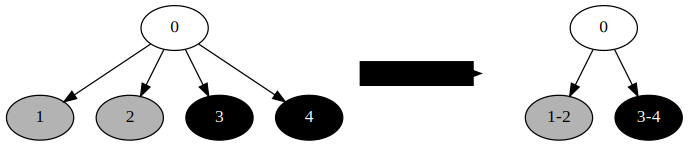
\includegraphics[width=0.7\textwidth]{algo_F2}
  \caption{Exemple d'agrégation avec l'opérateur F et le paramètre 2.}
  \label{fig:algo_F2}
\end{figure}

